%\chapter{Background and Related Work} \label{background}

This chapter covers the essential background and related work for subsequent chapters. Section \ref{sec:CE} begins with an introduction of causality extraction in the context of text mining. Three main approaches are described: 1. linguistic patterns and rule-based, 2. traditional ML based on manual feature selection, and 3. neural network-based deep learning models. Section \ref{sec:clustering} introduces basic concepts and techniques in NLP, such as word embeddings and compositional representations. Subsequently, text clustering algorithms based on these embeddings are discussed. Section \ref{sec:financial} provides an overview of related work with respect to text mining in financial reports, specifically, the Management Discussion and Analysis (MD\&A) section. Relevant SEC regulations are briefly introduced to provide a background understanding of the the formats and contents of these filings. Finally, Section \ref{sec:related} highlights a select few papers that are most relevant to this thesis.



\section{Causality Extraction} \label{sec:CE}

\subsection{What is Causality Extraction}

Causality Extraction (CE), also known as causality mining, is a subfield of Information Extraction (IE), which itself is a subfield of Text Mining \cite{Yang21Survey,Ali21Survey}. See Figure \ref{fig:CETaxomony} for an overview of the taxonomy of the field, highlighting the key topic of this thesis, i.e., Causality Extraction, with respect to other relevant subfields. 

\begin{figure}[h!]
\centering
  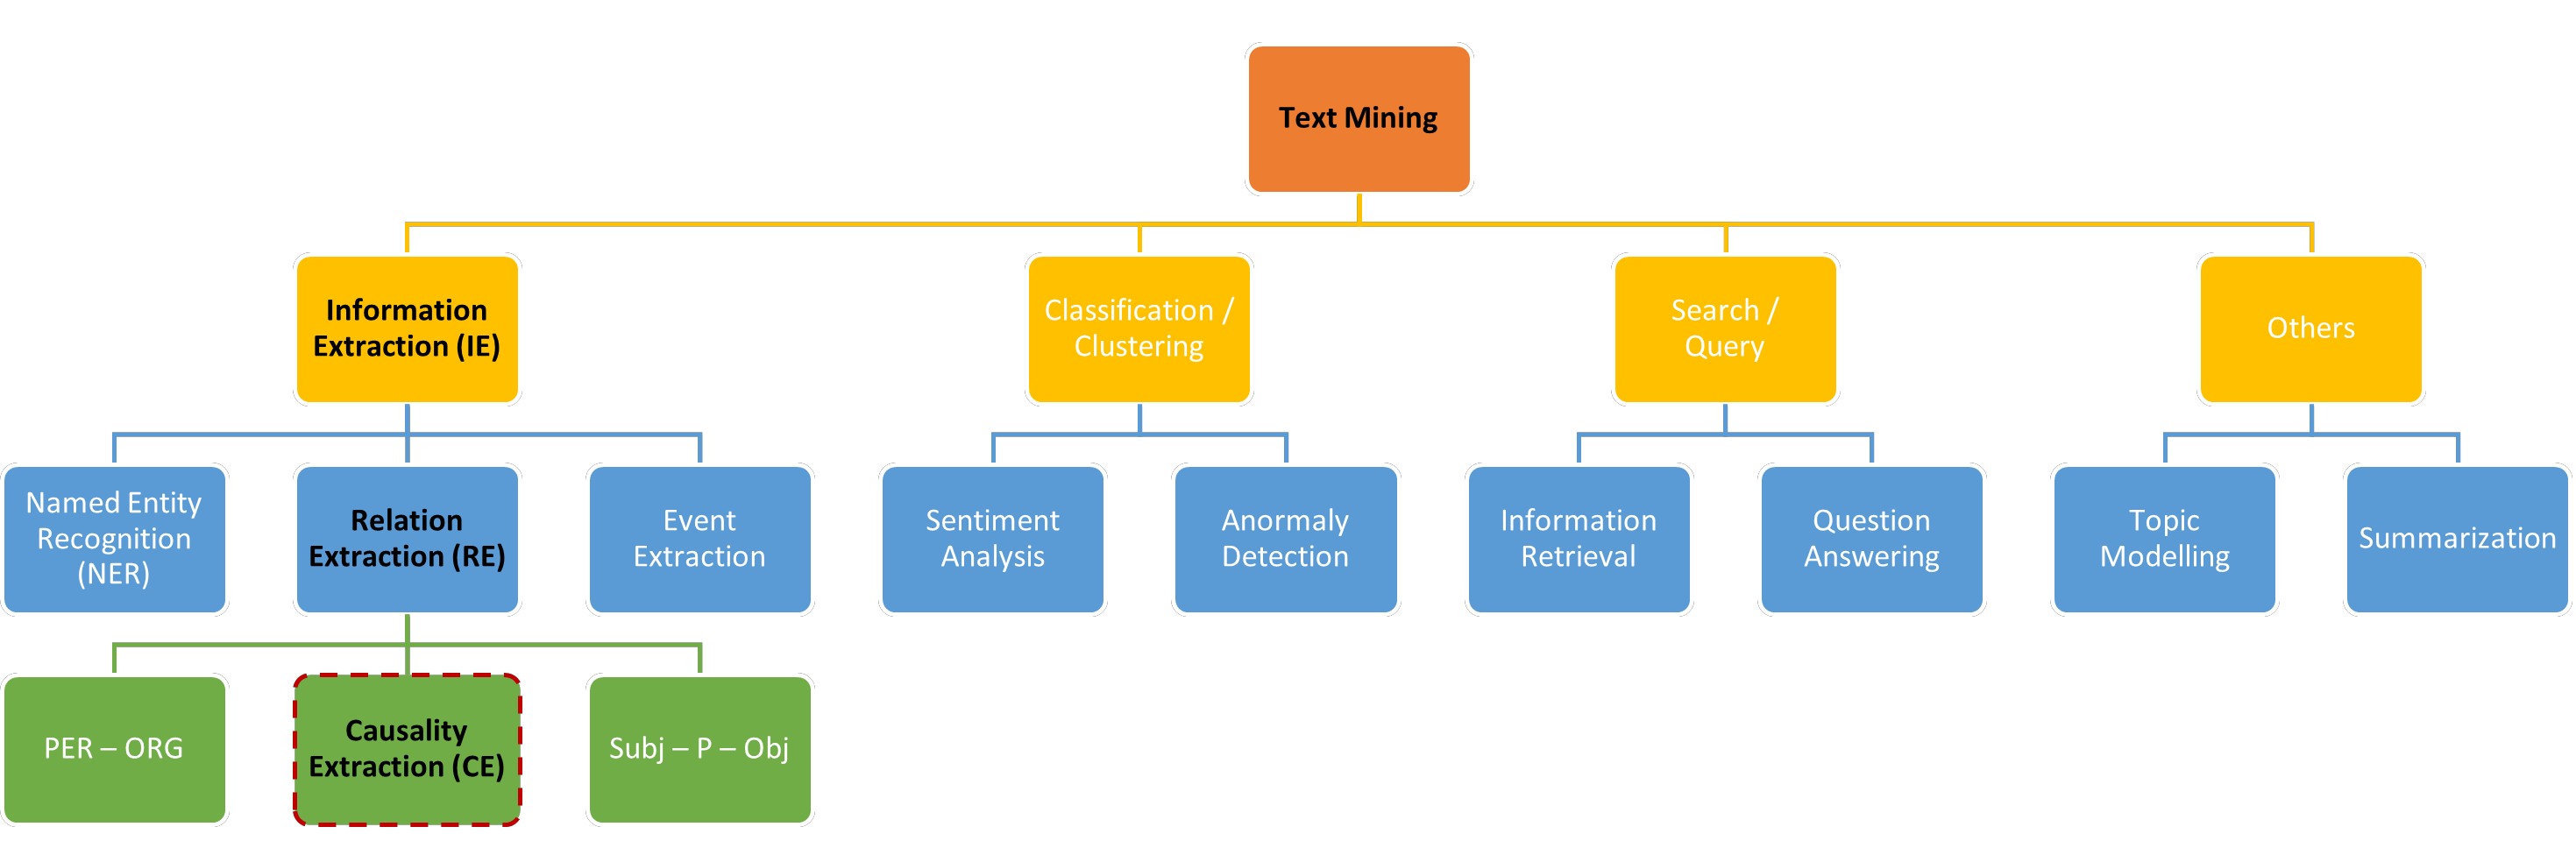
\includegraphics[scale=0.7]{figures/CETaxonomy.png}
  \caption{Causality Extraction's Position in the Taxonomy of Text Mining}
  \label{fig:CETaxomony}
\end{figure}


%[what is causality 0.5 page]
Causality is a type of relation between two events, states, phenomena or entities, in which one (referred as the \emph{cause}) triggers the other (referred as the \emph{effect}). Causal reasoning is the process of identifying causality. Understanding causality is a fundamental trait of human intelligence. We perform causal reasoning intuitively. However, it is often not a straightforward task to define what is \emph{cause} and what is \emph{effect}. The exact nature of \emph{cause} and \emph{effect} is indeed a metaphysical question that has sparked a long and deliberate philosophical debate which is still unresolved \cite{Ali21Survey}. 

Within the scope of this thesis, CE is defined in the context of NLP as the task of identifying the \emph{claimed} causal relation between a pair of events that are asserted in written texts \cite{causenet2020}, regardless of the nature and the validity of that relation in reality. In other words, there could be a disparity between the true causality in reality and the \emph{claimed} causality expressed in some given text. Due to the implicit nature of logic and the ambiguity of construction when expressing causal relations in natural language, it is a challenging task, for both humans and machines, to accurately identify exact causality \cite{DunietzThesis18}.


%[causality expression in language: explicit/implicit/ambiguous]
Causality can be expressed in a variety of ways in natural languages, using many different semantic representations and syntactic patterns. For example, it can be explicitly marked by certain words or phrases, such as \emph{because, due to, as a result of}, etc.  These words and phrases are often referred to as \emph{causal markers, causal links or causal connectives} \cite{KhooThesis95}. Causality can also be embedded in a sentence or a group of sentences in an implicit way. For instance, in the text \emph{"Thomas Cook's demise leaves its German operations hanging. More than 140,000 German holidaymakers have been impacted and tens of thousands of future travel bookings may not be honored."} \cite{FinCausal20}, the cause is in the first sentence and the effects are in the second sentence, however, there is an absence of explicit causal connectives linking the two. In addition, there can be cases where the causality is ambiguous and sometimes shared with other types of relations such as temporal, obligation, conditional dependence, etc. See examples in Table \ref{table:exampleSentences}  

\begin{table}[ht]
    \centering
	\begin{tabular}{{p{0.15\linewidth} p{0.6\linewidth} p{0.15\linewidth}}} 
		 \hline
		Connectives & Sentences & Causality \\
		 \hline\hline
		As & There was no debate \emph{as} the Senate passed the bill on to the House. & Causal  \\
		As & It has a fixed time, \emph{as} collectors well know. & Non-causal \\
		 \hline
		After & Bischoff in a round table discussion claimed he fired Austin \emph{after} he refused to do a taping in Atlanta. & Causal \\
		After & In stark contrast to his predecessor, five days \emph{after} his election he spoke of his determination to do what he could to bring peace. & Non-causal \\
		 \hline\hline
		\end{tabular}
	\caption{Examples of ambiguous causal connectives, sourced from \cite{Yang21Survey}}
	\label{table:exampleSentences}
\end{table}


Research in CE is not very well developed as compared with other subfields of NLP, such as machine translation, sentiment analysis, etc. Although it has gained traction in recent years, systematic studies and available datasets on causality are still rather limited \cite{Xu20Review}. Broadly speaking, CE is perceived as two subtasks by existing literature: 1) detection of whether a sentence contains a causal relation; 2) extraction of the relevant cause and effect chunks \cite{FinCausal20}. The first subtask is treated as a text classification problem and the second one a sequence tagging problem. 

\paragraph{Text Classification:} This category mainly concerns identifying whether a sentence contains a causal relation. It is typically framed as a binary classification aiming to distinguish causal sentences from non-causal ones. An additional subtask in this category is to determine the direction of causality. When a pair of chunks representing cause and effect is indicated in a sentence, the classifier also needs to discriminate the cause from the effect, i.e., this becomes a multi-class classification: cause-effect, effect-cause and non-causal. The majority of the existing studies belongs to this category \cite{FinCausal20, SemEval07Task4, SemEval10Task8}.

\paragraph{Sequence Tagging:} This category focuses on identifying the chunks in a sentence that represent cause, effect and causal connectives. This is usually treated as a sequence tagging task with a BIO-scheme (B: Beginning, I: Inside, O: Outside). The overall aim is to assign a tag to each word in the sentence. Figure \ref{fig:BIOtags} shows an example of such a tagging scheme \cite{Li21BiLSTMCRF}. Although this is also a classification task, the approach used is very different from Text Classification due to the presence of a sequence and the logical relationships between tags \cite{Ali21Survey, FinCausal20, Xu20Review}.

\begin{figure}[h!]
\centering
  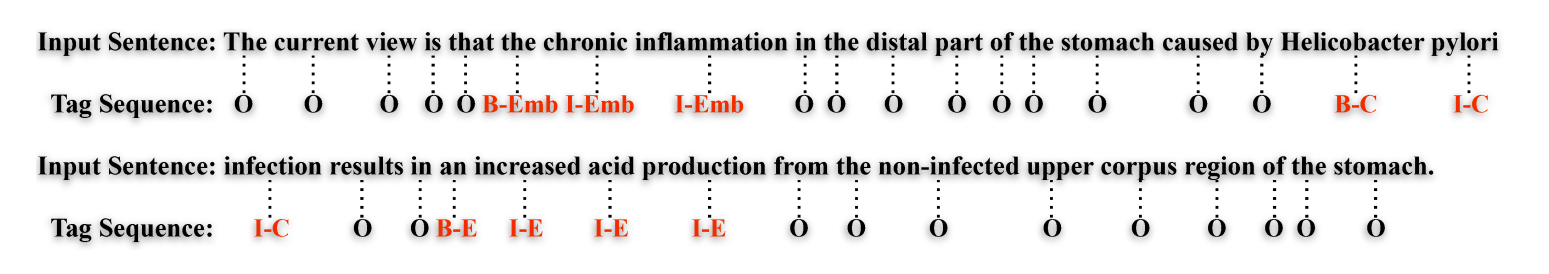
\includegraphics[scale=0.45]{figures/BIO.png}
  \caption{Illustration of Causality Sequence Tagging. Tag "O" represents the "Outside" or "None", which means that the corresponding word is irrelevant in any causality components. Tag "B-C" represents the "beginning of cause", tag "I-C" represents the "inside of cause", tag "B-E" represents the "beginning of effect", tag "I-E" represents the "inside of effect", tag "B-Emb" represents the "embedded causality begin", and tag "IEmb" represents the "embedded causality inside". Example sentence and tagging scheme taken from \cite{Li21BiLSTMCRF}.}
  \label{fig:BIOtags}
\end{figure}


\subsection{Techniques and Approaches}

% [Classification Approach: rule-based vs statistical ML vs NN/Deep Learning 2 pages]
In terms of techniques developed for CE, existing literature can be chronologically categorized into three stages: 1) linguistic pattern and rule-based approach; 2) traditional ML approach based on manual feature selection; 3) neural network-based deep learning approach. These approaches also echo the overall trends in NLP development, which has shifted from linguistic heuristics to statistical models, and now is moving increasingly towards the data-driven neural network architectures. Appendix \ref{appendix:CEpapers} shows a summary table of all the papers relevant to causality extraction reviewed for this thesis.



\subsubsection {\emph{1. Linguistic Patterns and Rule-based Approach}}

The focus of this particular approach is on cause and effect that is explicitly indicated in written English and only linguistic clues are used to identify causal relations. This method recognizes causal relations based on pre-defined lexico-semantic and syntactic patterns. These patterns can be expressed in terms of a sequence of words or syntactic categories that usually indicate the presence of a causal relation. 

The pioneering works developed by Khoo \cite{KhooThesis95,Khoo98,Khoo01} proposed three sets of such patterns: 1. patterns involving a causal link that links two phrases within a sentence (e.g., \emph{due to, because of}), 2. patterns involving a causal link that links two adjacent sentences (e.g., \emph{therefore, hence}), 3. patterns involving causal verbs and resultative constructions (e.g., \emph{cause, result in/from}). To identify causal relations in a document, a computer program locates all parts of the document that match with any of the linguistic patterns. "Slots" in these linguistic patterns indicate which part of the text is the cause and which the effect. For example, the pattern \emph{[effect] is the result of [cause]} indicates that the part of the sentence following the phrase \emph{is the result of} represents the \textbf{cause} and the part of the sentence preceding the phrase represents the \textbf{effect}.

Girju \cite{Girju02, Girju03} narrows the focus on the most frequently used causal verbs (e.g., \emph{cause, lead to, bring about}, etc.) and a specific lexico-syntactic pattern \emph{<noun phrase 1, verb, noun phrase 2>}. In contrast to Khoo's method where a whitelist of words have to be predefined manually, Girju's approach can automatically detect and acquire a list of verbs and verbal expressions, which is subsequently validated based on semantic constraints with the help of WordNet. In order to extract the corresponding cause and effect chunks, the model identifies noun phrases by matching the longest word sequence that is defined in WordNet as a concept. 

Similarly, Chan and Lam \cite{SEKE05} also include a WordNet-based component in their Semantic Expectation-based Knowledge Extraction (SEKE) framework for finding concepts synonymous to the extracted cause and effect phrases. This helps with disambiguation and also generates new causal patterns that were previously unseen. 

In order to minimize reliance on explicit pattern specification and achieve better generalization, Ittoo and Bouma \cite{IttooBouma11} develop a weakly supervised system that uses Wikipedia as a knowledge-base to automatically produce lexico-syntactic patterns. Using a bootstrapping method by taking some causal pairs (e.g., \emph{rain} and \emph{flood}) as seeds, their system first identifies causal links (e.g., \emph{leads to}) in Wikipedia that connect these seed pairs. It then selects the top $k$ most reliable causal link patterns to extract other candidate pairs (e.g., \emph{heat} and \emph{drought}) that are connected by the same causal link (i.e., \emph{leads to}). This recursive procedure of learning new patterns from seed and candidate pairs and vice-versa is repeated until some desired number of causal patterns have been harvested. Since their system does not rely on explicit causal markers or specified patterns, it can detect and extract implicit causal relations in texts. In addition, their lexico-syntactic patterns neutralize word order and morphological variations, in contrast to the conventional surface-strings from previous works.


\subsubsection {\emph{2. Traditional ML Approach based on Manual Feature Selection}}

One of the shortcomings of the linguistic pattern and rule-based approach is that it cannot distinguish causal and non-causal sentences that contain the same linguistic patterns or causal connectors. For example, both sentences (1) \emph{"It was the first time any of us had laughed since the morning began."} and (2) \emph{"He had to depend on himself, since he was miles away from others."} contain the connective \emph{"since"}, however, only (2) is causal whereas (1) is temporal. In order to disambiguate causal semantic relations from non-causal ones, a discriminative classifier is used. In this traditional ML approach, a classifier, such as Support Vector Machine (SVM), Maximum Entropy (ME), Naive Bayes (NB), and Logistic Regression (LG), is trained on the annotated dataset with hand-engineered features, such as word position, part-of-speech (POS) tags, verb voice, etc.

This approach quickly gains popularity in the research community \cite{Sorgente13}, thanks to two reputable datasets provided by SemEval (Semantic Evaluation)\footnote{SemEval is a series of international NLP research workshops sponsored by the the SIGLEX Special Interest Group. https://semeval.github.io/}. SemEval-2007 Task 4 \cite{SemEval07Task4} provides a dataset for classifying semantic relations between two nominals (i.e., nouns or noun phrases). However, the causal relation is only one out of seven relations within this dataset and there are only 220 relevant sentences with binary labels (52\% causal vs 48\% non-causal). SemEval-2010 Task 8 \cite{SemEval10Task8} provides a slightly larger dataset with 1,331 annotated causal sentences which are pronouncedly imbalanced (91\% causal vs 9\% non-causal). These tasks only emphasize the detection of causal relations in sentences as the pair of words representing cause and effect have already been identified and annotated in the dataset. 

Based on the SemEval datasets, Rink et al.~\cite{Rink10} train an SVM classifier based on lexical-syntactic features such as context words, hypernyms, POS, dependencies, distance, semantic roles, etc.  Sorgente et al.~\cite{Sorgente13} train a Bayesian classifier based on three sets of features: i) lexical features, i.e., context words between cause and effect; ii) semantic features, i.e., all hyponyms and synonyms of each sense of cause and effect reported in WordNet; iii) dependency features, i.e., the direct dependencies of cause and effect in the dependency parse tree.  Zhao et al.~\cite{Zhao16} propose a new feature obtained by computing the similarity of the syntactic dependency structure of sentences. They use a Restricted Hidden Naive Bayes (RHNB) learning algorithm to process features and the interactions between causal connectives and lexico-syntactic patterns.


\subsubsection {\emph{3. Neural Network-based Deep Learning Approach}}

With the prevalence of Deep Learning (DL), Neural Network (NN) models such as Convolutional Neural Networks (CNNs), Recurrent Neural Networks (RNNs), and variants of the latter like Long Short-Term Memory (LSTM) and Gated Recurrent Units (GRU), have been increasingly applied to causality extraction. The goal of this approach is to allow the model to automatically learn and extract useful features and minimize the reliance on NLP toolkits for feature acquisition \cite{Yang21Survey,Ali21Survey}.

Before the advent of DL models, the traditional ML approach is often used in combination with the linguistic-based approach. One popular strategy is to build a multi-stage pipeline in which the candidate spans for cause and effect are first identified using the linguistic patterns, then a shallow ML-based classifier is applied to distinguish which candidate pairs are causal vs. non-causal based on pre-selected features. There are two ways this approach can be improved by NN models: 1) replacing the traditional ML-based classifier with an NN-based deep learning model; 2) replacing the multi-stage pipeline with a DL model trained end-to-end with raw input, thus combining the two sub-tasks (extraction and classification) into one task (sequence tagging).

Kruengkrai et al.~\cite{Kruengkrai17} introduce a multi-column CNN to classify event causality. The primary input of their method is candidates such as "smoke cigarettes" and "die of lung cancer", and the task is to judge whether they express a proper event causality. Similarly, Li and Mao \cite{LiMao19} propose a knowledge-oriented CNN model that incorporates prior knowledge from lexical knowledge bases for causal relation classification. Their model consists of a knowledge-oriented channel and a data-oriented channel. The input to their model is a sentence marked with two target entities for causal relation identification. 

Dasgupta et al.~\cite{dasgupta18} propose a linguistically-informed recursive neural network architecture for automatic extraction of cause-effect relations from text. Their model consists of two stacked layers of bidirectional LSTM, enhanced with an additional linguistic layer, which extracts features such as POS tags, dependency tags, etc. The input to the Bi-LSTM unit is an embedding vector which is the composition of the word embedding representation (pre-trained GloVe) and the linguistic feature embeddings. The model is trained on a dataset of ca. 8,000 manually annotated sentences, where each word in a sentence is assigned one of four labels: \emph{cause, effect, causal connectives} and \emph{none}. 

Chen et al.~\cite{Chen20} propose another joint model consisting of two layers of Bi-LSTMs. The first layer serves as a sentence segmenter, which encodes each token in a sentence, classifies whether it belongs to a causal connective and splits the sentence into segments and connectives. The second layer is a relation classifier, where the hidden state of each segment is fed into another Bi-LSTM layer for judging whether there exists a causal relation between all pairs of segments within the sentence. Hence, their model is capable of finding nested causality structures. The sentence segmenter and causal relation classifier are jointly trained in the same network, based on 69,120 manually labelled sentences.

Li et al.~\cite{Li21BiLSTMCRF} propose a neural causality extractor with the Bi-LSTM-CRF model as the backbone, which can directly extract cause and effect without extracting candidate causal pairs and separately identifying their relations. They formulate causality extraction into a sequence tagging problem and combine Bi-LSTM with a multi-head self-attention mechanism. Extending the annotations of the SemEval 2010 Task 8 dataset, their training set consists of 4,450 sentences and contains 1,570 causal triplets.

Another approach is to leverage the contextulized embeddings from pretrained language models such as BERT \cite{BERT2018}. The top two performers in the FinCausal 2020 competition \cite{FinCausal20} both adopt this approach. The purpose of this task is to extract, in provided text sections, the chunks identifying the causal sequences and the chunks describing the effects. The winning model, NTUNLP \cite{NTUNLPL20}, uses a BERT-CRF system and a Viterbi decoder for span optimization. The second place winner, BERT-SQUAD \cite{GBE20}, uses an augmented system with heuristics for span. Both models are trained with a labelled dataset consisting of 1,579 causal sentences extracted from financial news articles. 


% [Comparison of Approaches and Limitation of Causality Extraction research 1 pages]
\subsection {Evaluation and Comparison}

%[Evaluation methods] 
\paragraph{Evaluation Metrics:} As many CE systems are defined as a binary classification task, the following four metrics \cite{Jurafsky2009} are commonly used in their evaluation:

\[Precision = \frac{TP} {TP + FP} \]
\[Recall = \frac{TP}{TP + FN} \]
\[F1 score = \frac{2 \times TP} {2 \times TP + FN + FP}\]
\[Accuracy = \frac{TP + TN} {TP + FP + TN + FN}\]

TP (true positive) is the number of correctly identified causal pairs. FP (false positive) is the number of incorrectly identified causal pairs. TN (true negative) is the number of correctly identified non-causal pairs, and FN (false negative) is the number of incorrectly identified non-causal pairs. 

For CE systems that are tasked to identify cause and effect chunks, evaluation is based on exact matches at the word level. In this case, recall is the proportion of words extracted by human judges that are also extracted by the computer program, and precision is the proportion of words extracted by the computer program that are also extracted by human judges. The recall and precision figures are usually averaged across all causal relations \cite{FinCausal20,Khoo98}.

\paragraph{Performance Comparison:} Comparing performance across studies is complicated by the fact that each paper uses different data sources to evaluate their models, as demonstrated in the Appendix \ref{}. That said, one can still make a few observations:

1. For the rule-based approach, the precision and recall metrics are generally low in comparison to the other two more recent approaches. It is difficult to manually construct explicit linguistic patterns that capture the full complexity of causal expressions in natural languages due to their many different forms and inherent ambiguity.

2. The traditional ML approach focuses only on the classification problem and the performance is not necessarily better than the earlier works of the rule-based systems. Its advantage is to eliminate the requirement of manually constructing linguistic patterns. However, it still has to rely on sophisticated feature-engineering which needs to be handcrafted. In addition, feature extraction by NLP tools, such as POS taggers, dependency parsers, named entity recognizers etc., is not perfect, resulting in error propagation that can further reduce the performance of ML-classifiers. 

3. The deep neural network approach offers the best performance to date. However, these neural network models typically require large amounts of labeled data to train on. It is costly and time-consuming to manually annotate sufficiently large training datasets. Currently, there are only a selected few of them (such as SemEval and FinCausal) available for training causal models. However, with only a few thousand labeled causal sentences, it is hardly convincing that they are large enough to train meaningfully deep neural networks with complex architectures.

This thesis has only reviewed a select number of representative papers in the field of causality extraction. By and large, we have excluded papers that focus on the biomedical domain and non-English text sources. For a more complete survey of various methods and datasets for causality extraction, see \cite{Yang21Survey, Ali21Survey, Xu20Review, Asghar16Survey}. 

%[how to argue simple rule-based approach is more suitable for practical problem solving rather than complicated ML supervised models that feed on labelled data which we don't have]

%\newpage


\section{Text Clustering} \label{sec:clustering}


Text clustering is a widely studied problem in Text Mining (see Figure \ref{fig:CETaxomony} for an overview of the taxonomy). The task concerns dividing texts content into different groups where similar texts are grouped together \cite{Aggarwal2012}. Text clustering is an important technique for many downstream applications, such as document organization, text summarization and information retrieval \cite{surveyDocClustering2015, surveyTextMining2017}. In particular for this thesis, text clustering is employed organize and index causal factors after causality extraction. This Section starts with an introduction of word embeddings (Section \ref{sub:wordembeddings}) and phrase embeddings (Section \ref{sub:phraseembeddings}), followed by a discussion of three clustering techniques based on these embeddings (Section \ref{sub:clusteringalgo}).

\subsection{Language Representation and Word Embeddings}\label{sub:wordembeddings}

Natural languages are an inherently discrete and symbolic representation of human knowledge \cite{Ferrone20Survey}. Most written languages are composed of words, which form sentences that, in turn, form paragraphs, discourses, and so on. This composition of symbols in words and of words in sentences follow certain syntactical and semantic rules \cite{Cartuyvels21Survey}. Human reasoning leverages the manipulation of symbols at a cognitive level, which leads to abstract thinking and generalization.

In order for computers to process natural language, string-based texts need to be transformed into numerical form, typically as vectors consisting of real numbers. This transformation process of mapping the discrete symbolic representation of words into a continuous representation in the form of real-valued vectors is called vectorization or embedding. Broadly speaking, there are two methods to accomplish this: the vector space model and statistical language modelling \cite{WordEmbSurvey19}.

\paragraph{Vector Space Model:} Generally attributed to Salton et al.~\cite{Salton75}, the Vector Space Model stemmed from the field of Information Retrieval in the 1970s. Essentially, it is an encoding procedure, whereby each document in a collection of documents is represented by an n-dimensional vector, with each element representing a unique term in that document. This results in a term-document matrix, where each element can be either binary (indicating presence or absence) or a real number (count). This representation can be further normalized by a weighting scheme such as Term-Frequency-Inverse Document Frequency (TF-IDF). One disadvantage of this method is that the vectors have high dimensionality, but are very sparse (i.e., most entries are zeros). The size of each vector corresponds to the size of the entire vocabulary in the corpus, thus making computation such as similarity comparison inefficient. Another shortcoming of this vector representation is that it completely ignores the order of the terms as they appear in documents, essentially treating each document as a set of terms, thus losing the syntactic information therein.

\paragraph{Statistical Language Modelling:} Statistical language models are probabilistic or neural network-based models of the distribution of words in a language. These models focus on predicting target words given $n$-number of preceding or surrounding words. This approach is based on the distributional hypothesis formulated in the 1950s by linguists like Joos \cite{Joos50}, Harris \cite{harris54}, and Firth \cite{firth57}. They observed that words have similar meaning if they are used in similar contexts. The idea is to represent a word as a point in a multi-dimensional semantic space that is derived from the distributions of neighbouring words \cite{Jurafsky2009}. These representations of words are effectively dense vectors, which represents the feature space of the underlying semantics. Their dimensionality is usually much smaller than the size of the vocabulary. These vectors are sometimes also referred to as \emph{word embeddings}. \emph{Embedding} is derived from the mathematical sense as a mapping from one space or structure to another. The term \emph{word embedding} was coined by Bengio et al. in 2003 \cite{Bengio2003}. There are many different types of word embeddings depending on the underlying probabilistic distribution models or neural architecture. A few important word embedding schemes, such as \emph{Word2Vec, GloVe, BERT}, etc., are described and discussed below. 

\subparagraph{\emph{Word2Vec:}} Mikolov et al.~\cite{w2v2013} created word2vec, a toolkit for training and applying pretrained embeddings. A \emph{Word2Vec} model is a simple two-layer feed-forward neural network. It takes a large text corpus as its input and outputs a set of vectors representing the words in the corpus. The resulting vector space is typically of several hundred dimensions, and it is positioned such that words that share common contexts in the corpus are located in close proximity to one another in the space. Depending on how the embeddings are learned, there are two different architectures of the \emph{Word2Vec} model: (1) the continuous-bag-of-words (CBOW) model predicts the target word using the context words; and (2) the skip-gram model uses the target word to predict the context words. Effectively, CBOW and Skip-Gram are inverses of each other. Trained on the Google News dataset (about 100 billion words), \emph{Word2Vec} is one of the most popular pretrained word embeddings. Standard \emph{Word2Vec} models are not able to assign vectors to out-of-vocabulary words and instead use a default vector that reduces their predictive value.

\subparagraph{\emph{GloVe:}} Pennington et al.~\cite{glove2014} released the Global Vector Model (GloVe), which is an unsupervised learning algorithm developed at the Stanford NLP lab. It learns vector representations for words based on the aggregated global word-word co-occurrence statistics from a corpus. The main intuition is that the ratios of co-occurrences encode actual semantic information about pair of words. \emph{GloVe} creates a global co-occurrence matrix by estimating the probability a given word co-occurs with other words. The loss function is the difference between the product of word embeddings and the log probability of co-occurrence ratios. \emph{GloVe} embeddings have been pre-trained on the Common Crawl dataset with 42B or 840B tokens and a vocabulary of 1.9M or 2.2M tokens, Wikipedia 2014 + Gigaword 5 with 6B tokens and a vocabulary of 400K tokens, as well as Twitter using 2B tweets, 27B tokens and a vocabulary of 1.2M tokens.


Both \emph{Word2Vec} and \emph{GloVe} are word-level embedding models. In contrast, there are other types of embedding models, such as \textbf{\emph{ELMo}} and \textbf{\emph{Flair}}, which produce character-level embeddings. \emph{ELMo} (Embeddings from Language Models) \cite{elmo2018} is a deep bidirectional language model that produces character-based word vectors from its internal states. ELMo claims that lower-level LSTM states capture aspects of syntax, while higher-level states model aspects of word meaning in context. It has proven its success on different tasks such as question answering (QA), semantic role labeling (SRL) and named entity recognition (NER). \emph{Flair} \cite{flair2019} is a context-sensitive model. Similar to \emph{ELMo} it leverages the internal states of a trained language model, but uses characters as atomic units for a one-layer biLSTM. \emph{Flair} is trained without any explicit notion of words and at each point in the sequence predicts the next character. 

\subparagraph{\emph{BERT:}} \emph{BERT} is a contextual language model released by Google Research in 2018 \cite{BERT2018}. It is based on the Transformer architecture and the attention mechanism that learns contextual relations between words and sub-words. Pretrained on Wikipedia and BooksCorpus with the combined objectives of masked language modeling and next sentence prediction, \emph{BERT} can be adapted to various downstream NLP tasks. BERT is open source and various pretrained versions (e.g. base vs large, cased vs uncased, multi-lingual, etc.) are available for download directly from Hugging Face. 

There are several differences between word-level embedding models, such as \emph{Word2Vec} and \emph{GloVe}, and contextual language models, such as \emph{BERT}. One key difference is that the former generate static vectors, whereas the latter generates dynamic vectors. For example, \emph{BERT} generates different vectors for the same word, depending on the context of the input sentences. On the other hand, a pretrained \emph{Word2Vec} model generates the same vector for the same word, regardless of its context. This one-to-one mapping with a single indexing operation makes the pretrained word vectors from \emph{Word2Vec} and \emph{GloVe} models computationally more efficient to deploy in downstream applications. In contrast, in order to obtain the word embedding from the \emph{BERT} model, both the word and its context sentence are required as input. The model generates word vectors dynamically as the same word appears in different contexts. As a result, the transformer-based neural models are harder to deploy in production due to their higher computational intensity. 



\subsection{Compositional Representation and Phrase Embeddings}\label{sub:phraseembeddings}

Language is by nature compositional. Words form phrases and subsequently sentences. Concatenative compositionality is the ability of a symbolic representation to describe sequences or structures by composing symbols with specific rules \cite{Ferrone20Survey}. In this process, symbols remain distinct and composing rules are clear. To capture the meaning of phrases in vector forms, there are two main approaches to phrase representations: non-compositional and compositional \cite{NPcomposing19}. The non-compositional approach treats phrases as single units (as if they were words), and learns phrase representations directly from corpora. However, this approach is not scalable for all possible phrases due to the combinatorics of component words. In contrast, the compositional approach derives a phrase representation from the embeddings of its component words. 

There are many different methods for computing phrases representations from word vectors, such as simple addition and average operations \cite{Mitchell2010}, matrix-vector composition operations \cite{baroni-zamparelli-2010,zanzotto2010} and rule-based composition using features to capture phrase structure and context \cite{yu-dredze-2015}. However, such approaches often ignore word order and other linguistic intuitions \cite{zhu18sentence}. Recently, more complex neural network architectures have been explored to learn a non-linear composition function that combines component word embeddings together into a single phrase embedding. This function has been implemented with RNN models such as GRU \cite{zhou17} as well as transformer-based models such as \emph{PhraseBERT} \cite{PhraseBERT21}.

There is also an interesting observation in the literature that is worth noting. White et al.~\cite{White2015}, Wieting et al.~\cite{Wieting2016} and Arora et al.~\cite{Arora2017} found that simple operations outperform complex deep architectures. Furthermore, Reimers and Gurevych \cite{sentenceBERT2019} and Li et al.~\cite{sentenceEmb2020} found that without task-specific fine-tuning, the performance of \emph{BERT} on phrases and sentences is often worse than simple baselines such as mean-pooling over \emph{GloVe} vectors. 


\subsection{Clustering Algorithms}\label{sub:clusteringalgo}

Clustering is an unsupervised machine learning technique that aims to separate unlabeled data into different groups. According to \cite{Jain2010}, the operational definition of clustering can be stated as follows: given a representation of $n$ objects, find $K$ groups based on a measure of similarity such that the similarities between objects in the same group are high while the similarities between objects in different groups are low. Clustering has been widely used in data analysis to gain insight into the underlying structure of data distributions and help detect anomalies or outliers. Furthermore, it is also used as a compression method for summarizing data through cluster prototypes \cite{Jain2010}. 

There are many different algorithms to perform clustering. Xu et al.~\cite{Xu2015Survey} provide a comprehensive survey, summarizing the commonly used clustering algorithms into 19 categories. Three key clustering algorithms, partition-based K-means, hierarchy-based Brown Clustering and model-based Self Organizing Maps are discussed below.

\paragraph{K-Means:} K-means is a partition-based clustering algorithm that aims to find an optimal data partition such that the sum of squares of distance between the center of a cluster and all data points belonging to the cluster is minimized. Let $X ={x_i}, i = 1, ... , n$ be the set of $n$ $d$-dimensional points to be clustered into a set of $K$ clusters, $C = {c_k}, k =1, ... , K$. Let $\mu_k$ be the mean of cluster $c_k$. The squared error between $\mu_k$ and the points in cluster $c_k$ is defined as: 
\[J(c_k) = \sum_{x_i \in c_k} ||x_i - \mu_k||^2 \]
The goal of K-means is to minimize the sum of the squared error over all $K$ clusters: 
\[J(C) = \sum_{k=1}^{K} \sum_{x_i \in c_k} ||x_i - \mu_k||^2 \]

The main steps of the K-means algorithm are as follows \cite{Jain2010}: 
\begin{enumerate}
  	\item Select an initial partition with K clusters. 
	\item Generate a new partition by assigning each data point to its closest cluster center. 
	\item Compute new cluster centers.
	\item Repeat steps 2 and 3 until cluster membership stabilizes.
\end{enumerate}

K-means requires a pre-determined $K$ in order to initialize the centroids in Step 1. Next, the rest of the data points are assigned to their nearest centroids. Then, a new set of centroids are computed based on the mean of the assigned data points in the clusters. These two steps are done iteratively until the centroids stop making notable movement. The distance metric used in K-means is Euclidean Distance. 

%{Minibatch K-means Clustering:} 
Minibatch K-means is a variant of the standard K-means algorithm. The main idea is to use small batches of a random subset of the data for each training iteration, instead of the complete dataset. Each minibatch updates the clusters and this is repeated until convergence is achieved. The empirical results suggest that the computation time of the minibatch k-means algorithm is greatly reduced while the difference between the quality of clusters is reported to be only a little less than the original standard k-means algorithm \cite{miniKmeans2013}.


%[limitations] 
K-means is often the default algorithm applied in most clustering projects due to its simplicity. However, apart from the fact that $K$ is often hard to choose in an unsupervised scenario, K-means does not scale well when the dimensionality of the data is too high or the intended clusters are of varying size or density. 

%[Elbow methods] In this approach, the number of clusters $K$ has to be fixed a priori. Therefore K-means algorithm is run multiple times for each $K \in [2, \sqrt{N}]$, where $N$ is the number of samples. The best number of clusters $K^*$ can be selected based on the Elbow Method [citation needed]. 



\paragraph{Hierarchical Clustering:} Hierarchical clustering algorithms recursively find nested clusters either in agglomerative mode or in divisive mode \cite{Jain2010}. Agglomerative clustering is a bottom-up approach which starts with each data point in its own cluster and merges the most similar pair of clusters successively to form a cluster hierarchy. In contrast, the top-down divisive mode starts with all the data points in one cluster and recursively divides each cluster into smaller clusters. The output of hierarchical algorithms is a tree-like structure called a dendogram (see Figure \ref{fig:brownclustering} for an illustration). This structure can be segmented at different levels to give different corresponding clusters. 

\begin{figure}[h!]
\centering
  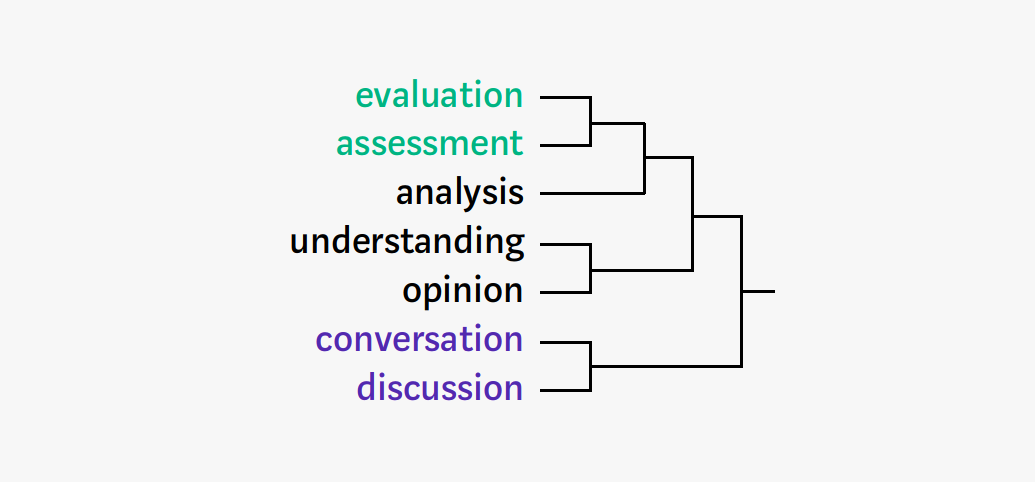
\includegraphics[scale=0.4]{figures/BrownClustering.png}
  \caption{Illustration of a dendogram from Brown Clustering. Adapted from \cite{Brown1992}}
  \label{fig:brownclustering}
\end{figure}

Brown clustering \cite{Brown1992} is an instance of the agglomerative hierarchical clustering algorithm. It uses mutual information based on distributional similarity to place similar words in the same cluster and similar clusters nearby in a binary tree \cite{Derczynski2015}. In practice, Brown clustering takes an input corpus $T$ and number of classes $K$, and uses mutual information to assign each term in the corpus vocabulary $V$ to one of the $K$ classes. Ideally, each class contains highly semantically-related words, by virtue of words being distributed according to their meaning. In the main implementation of Brown clustering \cite{Liang2005}, mutual information is measured at the bigram level. 

Brown clustering is a greedy algorithm. Its high computational complexity, together with a lack of efficient implementations, limits its applicability in NLP \cite{ciosici2020}. In addition, Brown clustering essentially works at the word-level and there is no known adaption to phrases.



\paragraph{Self-Organizing Map:}
%[What is it?] 
Self-organizing map (SOM) is an unsupervised learning technique that map multidimensional data onto lower dimensional subspaces via a neural network. First proposed in 1982 by Kohonen \cite{Kohonen1982,Kohonen2001}, it is also known as the Kohonen network. Often used as a data visualization technique, SOM takes $n$-dimensional input data and outputs a two-dimensional map, which resembles a landscape where regions can be interpreted as clusters and the geometric closeness between clusters also indicates their similarity.
 
%[What’s the procedure?] 
A simple SOM is essentially a feed-forward neural network trained with a competitive learning algorithm. Typically, it consists of a two-dimensional grid of nodes. Each node is initialized to be a randomly-generated weight vector of the same dimensions as the input data. During training, an input is presented to the network, and the node that is most similar to this input is selected to be the 'winner'. The winning node is then updated towards the input vector under consideration. Other nodes in the neighborhood are also influenced by the input vector in a similar manner, but as a function of their topological distance to the winner. The final output of a SOM is such that adjacent nodes have a greater degree of similarity to each other in comparison to nodes that are far apart. In this way, the SOM extracts the latent structure of the input space.

An illustration of the SOM with a two-dimensional grid view is provided in Figure \ref{fig:SOM}. The steps of the SOM learning algorithm are as follows:

\begin{enumerate}
  	\item \emph{Initialize:} Select the grid size (i.e., $X \times Y$), topology (e.g., rectangular), neighborhood function (e.g., Gaussian) and learning rate; each neuron is initialized with a random weight vector that has the same dimension as the input data. 
	\item \emph{Sample:} Select an input data point at random and feed it into the SOM.
	\item \emph{Match:} Find the Best Matching Unit (BMU), which is the neuron with the weight vector most similar to the input data. The similarity measure is usually based on Euclidean distance. 
	\item \emph{Update:} Adjust the weight vectors of the BMU and its neighboring neurons to be closer to the input data according to the preset neighborhood function and learning rate.
	\item Repeat steps 2 - 4 until the neuron weights stabilize.
\end{enumerate}


\begin{figure}[h!]
\centering
  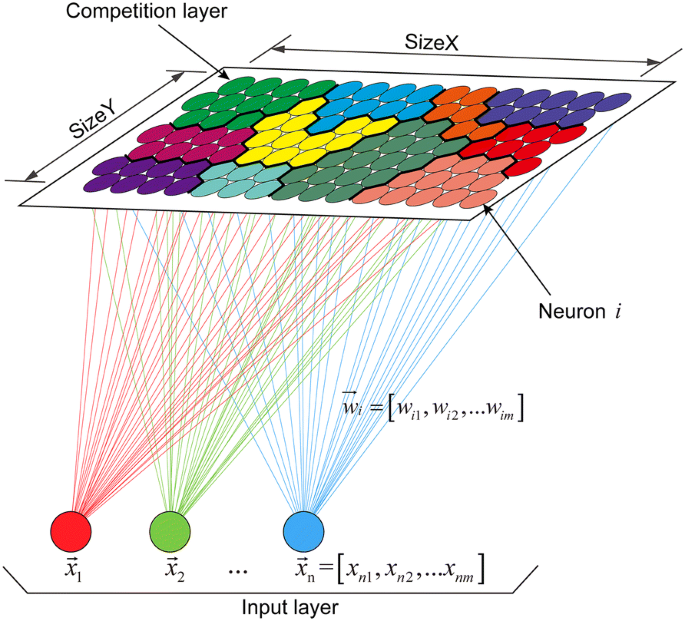
\includegraphics[scale=0.4]{figures/SOM_1.png}
  \caption{Illustration of a SOM. Adopted from \cite{Han2019}}
  \label{fig:SOM}
\end{figure}


%[add evaluation measures of SOM]
Kohonen originally suggested to use quantization error (QE) as the basic quality measure for evaluating SOMs \cite{Kohonen2001}. It is a measure of the average distance between the data points and the map nodes to which they are mapped, with smaller values indicating a better fit \cite{SOM2017}. The QE value for a SOM model is calculated using Equation \ref{qe}, where $n$ is the number of data points in the training data and $\phi : D \rightarrow M$ is the mapping from the input
space $D$ to the SOM $M$:

\begin{equation}\label{qe}
QE(M) = \frac{1}{n} \sum_{i=1}^{n} || \phi (x_i) - x_i||
\end{equation}

Topographic error (TE), on the other hand, is a measure of how well the structure of the input space is modeled by the map. It accounts for a SOM's preservation of local topological features in a low dimensional output space \cite{SOM2017}. Specifically, it is calculated according to Equation \ref{tp} by finding the best-matching and second-best-matching neurons in the map for each input and then evaluating their positions. If the nodes are next to each other, then topology is deemed to have been preserved for this input. If not, then this is counted as an error. The total number of errors divided by the total number of data points gives the topographic error of the map.  

\begin{equation}\label{tp}
TE(M) = \frac{1}{n} \sum_{i=1}^{n} t(x_i)
\end{equation}

where $t(x) = 0$ if the best matching and second best matching neurons are neighbors; else $t(x) = 1$.

% In each epoch, the SOM model is updated the same number of iterations as the number of data points in the training set, as the model is presented with only one data point in each iteration. As shown in Figure \ref{fig:epoch}, we find that increasing number of epochs (i.e. number of times that the model is trained on the entire dataset) does not affect the quantization error and the topographic error.


%[Limitations and applications] 
SOM has a few limitations. One drawback is that unlike other cluster methods, it has no distinct cluster boundaries. When datasets become more complex it is not easy to distinguish the cluster by pure visualization \cite{SOM2016casestudy}. SOM also suffers from the following problem: the network structure including the topology and the number of units has to be set before training and different structures lead to different results \cite{SOM2003}. 

%Evaluation of clustering: 
Clustering remains as a difficult problem in a number of application domains. This can be attributed to the inherent vagueness in the definition of a cluster, and the difficulty in defining an appropriate similarity measure and objective function \cite{Jain2010}. Ideally, clusters are isolated and compact. In reality, the determination of a good cluster is subjective and depends on its end application. Its significance and interpretation often requires domain knowledge. However, while humans are excellent cluster identifiers in two to three dimensions, automatic algorithms are needed to process higher dimensional data \cite{Xu2015Survey}. 



\section{Text Mining in Financial Reports}\label{sec:financial}

\subsection{SEC Regulation} \label{subsec:SEC}

% [SEC regulation and financial documents format 1 page]
The Securities and Exchange Commission (SEC) is the regulatory body in the United States whose mission is to facilitate a fair, efficient and transparent market. The SEC requires all publicly-listed firms in the U.S. to comply with certain disclosure requirements. This information is published in electronic form through the Electronic Data Gathering, Analysis and Retrieval System (EDGAR). EDGAR is a public database offering free access to professional and retail investors alike to research a public company's financial information and operations by reviewing the filings the company makes with the SEC. The system processes about 3,000 filings per day, serves up 3,000 terabytes of data to the public annually, and accommodates 40,000 new filers per year on average.\footnote {https://www.sec.gov/edgar/about} 

The sheer volume and frequency of information uploaded to EDGAR makes it impossible for human experts to manually scrutinize all available and potentially relevant content. Unsurprisingly, practitioners increasingly turn to technological solutions for assistance. However, automatic information extraction is a challenging task for machines due to the myriad filing forms and heterogeneity of file types. With a list of over 150 filing forms, EDGAR contains thousands of document types, both structured and unstructured, across many file formats such as HTML, PDF, plain text, PowerPoint, event pictures, images, etc. \cite{OpenEDGAR2008}.

The SEC has made a number of changes to its file format requirements since its founding in 1933. Its electronic repository dates back to 1984. As a result of this long history, there are no consistent file types even for the same type of forms in the EDGAR database. For example, SEC has initiated the eXtensible Business Reporting Language (XBRL) for the EDGAR database in 2005, in order to facilitate automated information extraction. In XBRL, filers tag their financial statements with elements from a taxonomy that defines the reporting concepts so that the accounting numbers are linked and can be collected automatically. Early adoption of XBRL by companies was gradual, but it was finally made mandatory in 2014. In 2018, the SEC adopted new rules requiring financial information to be submitted in the Inline XBRL format. Inline XBRL is a specification of XBRL that is both human-readable and machine-readable.\footnote {https://www.sec.gov/page/osdhistoryandrulemaking} 

Furthermore, companies have considerable flexibility in changing the tagging, wording, and presentation of these documents as long as they follow a predefined reporting structure. Loughran et al.~\cite{Loughran2016} pointed out a few issues, for instance, the 10-K filings are far less structured prior to about 2002 and many times a segment is mislabelled or misspelled. As a result, what seems like an obvious segmentation of the document, computationally is not. In addition, the same types of SEC filings may vary significantly between companies and over time, prohibiting researchers, regulators, and even many well-equipped practitioners from utilizing automation to extract information \cite{lazyprices2020}.

Despite these challenges, corporate disclosures on EDGAR are still a very important data resource for academic research, especially for longitudinal studies that requires historical data going back many decades. With regards to studies in Finance and Accounting, many recent survey papers have pointed out that the most commonly used datasets for text mining analyses are annual reports (Form 10-K) and quarterly reports (Form 10-Q) \cite{Tueregun2019, Gupta2020, Ravula2020}. In particular, within these 10-K and 10-Q filings, the Management Discussion and Analysis (MD\&A) sections are the focal point for many studies.

\subsection{Management Discussion and Analysis}

MD\&A is a narrative explanation of the financial statements and other statistical data that the registrant believes will enhance a readers' understanding of its financial condition, changes in financial condition and results of operation\footnote{https://www.sec.gov/corpfin/cf-manual/topic-9}. The SEC and the International Accounting Standards Board (IASB) insist on providing meaningful causal explanations and related discussions of performance results in management commentary.

The SEC specifically requires that the MD\&A section "should not consist merely of numeric dollar and percentage changes measured from period to period. [...] The focus should be on an analysis of the factors that caused these changes to occur."\footnote {https://www.sec.gov/corpfin/cf-manual/topic-9} For example, if sales declined because the volume of goods sold decreased by 20\%, but this was offset by a 10\% increase in price, the discussion in MD\&A should not stop once it identifies the price and volume components. In this example, the underlying factors that contributed to the decline in volume as well as the increase in selling prices should also be discussed. It is further suggested that for events that are likely to cause a material change in the relationship between costs and revenues (e.g., increases in labor costs or raw materials), the change in the relationship should be disclosed.
 
In its Practice Statement, the IASB (2010)\footnote {https://www.ifrs.org/issued-standards/list-of-standards/management-commentary-practice-statement/} voices similar arguments. Firms should use management commentary to include their own perspective on how their business is evolving with an analysis of how different factors are interacting to assist market participants in interpreting the financial statements and in comprehending their content in relation to management's objectives and strategies and action to achieve those objectives. Causal reasoning about performance is imperative in this respect \cite{Zhang2018}.

There are many studies focused on MD\&A, though causality-related research is rare. Clarkson et al.~\cite{clarkson1998} present evidence regarding the usefulness of MD\&A. and on disclosure quality. Numerous research analyzes MD\&A to explain a company's M\&A strategy (\cite{Ahmed2016}), future earnings and profitability (\cite{Feldman2010, Bochkay2014, AmelZadeh2016}), stock performance (\cite{AmelZadeh2016, TaoDeokar2018}), bankruptcy and litigation risks etc. (\cite{YangDollarMo18, BourveauLouWang18}). Most of these studies focus on basic and simple indicators such as readability, FOG index, tone and sentiment analysis, in combination with regularized regression methods to explain correlation between a company's attributes and its financial disclosure. Ravula \cite{Ravula2020} provides a very comprehensive summary of all latest research in this field and points out that text analysis in finance is still in the early stages.

Separately, MD\&A has also been used as a domain specific corpus to train language models. FinBERT \cite{finBERT2020} obtains 60,490 Forms 10-K and 142,622 Forms 10-Q of Russell 3000 firms for 1994 to 2019 from the SEC's EDGAR website. 

%There are also knowledge graph construction related studies. Such as company holdings, management employment, competitor analysis, etc. [add reference]


% TODO
\section{Related Work} \label{sec:related}
Most of the works mentioned in the previous sections of this chapter are relevant to this thesis. In this section, we highlight a select few that are the most relevant. They all use financial filings as their main corpra to extract information. 

Zhang et al.~\cite{Zhang2018} use automated techniques to measure causal reasoning on earnings-related financial outcomes of a large sample of MD\&A sections of US firms. They find a positive and significant correlation between a company's causal reasoning intensity and the earnings forecast accuracy by analysts following the company. One limiation of this study is that they use a rather simplistic approach to measure the causal reasoning word intensity, i.e., by counting the relative frequency of causal reasoning words in the performance-related paragraphs of the MD\&A. The identification of the causal reasoning words is based on a list of causal words used by Linguistic Inquiry and Word Count (LIWC). 

Chen et al.~\cite{Chen20} use financial statements as the corpus to extract nested causality. They propose to train a joint model consisting of two layers of Bi-LSTMs end to end based on the annotated dataset. Their model is capable of finding nested causality structure in a sentence. The first layer of the model separate a sentence into segments and the hidden state of each segment is fed into the second bi-directional LSTM layer, which classifies whether there exists a causal relation between all pairs of segments within the sentence. To train this neural network, significant effort is required to prepare the data for manual annotation. In their case, a team of 25 volunteers participated in the annotation task. They manually collected and annotated 69,120 sentences from 2,039 published financial documents. Unfortunately, neither the source of the financial documents nor the language of these documents is specified in the paper. Another limiation is that the authors did not make this annotated dataset publicly available, thus it cannot be used as a training set for this theisis. 

Cavar and Josefy \cite{MappingKG2018} uterlize NLP techniques to extract information from SEC filings and construct a knowledge graph of how companies, their executives and directors are linked to one another. Their graph-mapping approach includes extracting subject-predicate-object tuples from raw text and validating the semantic relations through linguistic analyses. However, due to the lack of a gold standard corpus or data set, the authors did not provide any formal and quantitative measure for the effectiveness of their extraction pipeline. In addition, another limiation is that this paper does not provide any overview of statistics on the final knowledge graph constructed, or how it can be used in downstream applications. 

Jen \cite{CompanyKG2021} constructs a company domain-specific knowledge graph that contains company-related entities and relationships, such as competitiors, subsiddiearies, suppliers and custerms, from 10-K filings. This project applies hybrid methods combining a pre-trained statistical model for NER and rule-based patterns for RE. To evaluate the proposed model's performance, the author manually gathers all the available triples based on the ontology schema from 10-K filings as a gold standard. Ten 10-K filings are used to create rule-based patterns and the system's performance is evaluated on another ten 10-K filings. A precision of  75.7\% and a recall of 53.6\% are achieved by the proposed system. As the data source only includes 20 filings, the scope of this project is rather limited. In addition, there is also no evaluation on possible end applications using the company domain-secific knowledge graph created. 

In addition to the works related to information extraction from financial documents, this thesis also borrows inspiration from the following paper, in terms of output visualiazation. Skupin et al.~\cite{SOM2013} implement a high-resolution visualization of the medical knowledge domain using the self-organizing map method, based on a corpus of over two million publications. They use a basic vector space model with a vocabulary consisting of only the top 10\%, or 2,300 most used MeSH terms (PubMed Medical Subject Headings) in conjunction with a large SOM consisting of over 75,000 neurons. After training, a neuron label clustering method is applied to merge boundaries and determine cluster labels. The resulting map is further annotated and evaluated by ten experts stemming from the biomedical domain. This study produces some very interesting visualization as output and concludes that it is possible to transform a very large document corpus into a map that is visually engaging and conceptually stimulating to subject experts.







